\chapter[Análise dos Resultados]{Análise dos Resultados}
\label{chap:Status}
Neste capítulo são apresentados os resultados obtidos através dos testes de usabilidade e experiência de usuário realizados no aplicativo Multilind. Os testes seguiram a estrutura de uma pesquisa-ação, que envolve a concepção e a realização de uma 
investigação em associação com a ação ou resolução de um problema conhecido, como descrito no \hyperref[sec:Metodologia de Analise de Resultados]{Capítulo 4}. No decorrer da análise de resultados, destacam-se as personas envolvidas, as funcionalidades 
testadas e práticas adotadas durante o protocolo de pesquisa-ação. Por fim, são apresentadas as considerações finais acerca dos resultados obtidos.

\section{Personas}
\label{sec:Personas}
Como descrito no Capítulo \hyperref[sec:Persona]{2}, as personas são representações semifictícias que detêm perfis desejáveis para os testes nos aplicativos. Esses perfis são definidos por características específicas que orientam a seleção da amostra, 
garantindo a consistência dos resultados. 

Com o intuito de avaliar a usabilidade e a experiência do usuário no aplicativo Multilind, foram realizadas provas de conceito para ambas as versões do aplicativo: a última versão (v1.4.0) e a versão com melhorias propostas. Para esse propósito, 
foram selecionados cinco usuários que representam diferentes perfis de personas, permitindo uma avaliação abrangente.

A escolha de cinco usuários orienta-se por uma abordagem amplamente adotada. \citeonline{usabilitytest} argumenta que realizar testes com cinco usuários é suficiente para identificar a maioria dos problemas de 
usabilidade. Ele baseia essa conclusão em estudos empíricos e observações, sugerindo que a descoberta de problemas de usabilidade tende a estagnar após o quinto participante, com poucos benefícios 
extras sendo obtidos com participantes adicionais.

O primeiro ciclo de testes foi realizado com objetivo de coletar métricas e informações de usabilidade e experiência do usuário no aplicativo Multilind implantado. Já o segundo ciclo de testes visou validar as 
melhorias propostas, no intuito de obter insumos, via análise dos resultados obtidos, sobre a pertinência dessas melhorias, na visão do público alvo. Dependendo do grau de concordância dos usuários, se alto, a 
melhoria é vista como pertinente, sendo mantida no plano de ação de melhorias a serem implementadas efetivamente no aplicativo. Em caso de baixa concordância, vistas como não pertinentes. Portanto, removidas 
do plano de ação de melhorias. Em caso de concordância parcial (ou seja, de grau intermediário), há adequação das melhorias considerando os apontamentos conferidos. 

Todos os participantes participaram voluntariamente, de acordo com os termos estabelecidos no  TERMO DE CONSENTIMENTO LIVRE E ESCLARECIDO (TCLE), que foi adaptado do modelo da Universidade de Araraquara \cite{tcle}, 
disponível no Apêndice \ref{ApendiceB} para consulta.

\section{Cenários de Uso}
\label{sec:Cenários de Uso}
Durante os ciclos de testes de usabilidade, foram avaliadas sete funcionalidades principais do aplicativo Multilind. Essas funcionalidades foram escolhidas com o objetivo de identificar os aspectos-chave do 
aplicativo. Os participantes foram solicitados a interagir com cada uma dessas funcionalidades e fornecer feedback instantâneo sobre suas percepções. As funcionalidades testadas incluem:

\begin{itemize}

	\item Visualizar línguas através do mapa (F01): Os usuários podem visualizar as diferentes línguas representadas geograficamente no mapa do aplicativo.

    \item Ver detalhes de uma língua ao clicar em um ponto no mapa (F02): Ao clicar em um ponto específico no mapa, os usuários podem acessar informações detalhadas sobre uma língua específica.
    
    \item Visualizar línguas por ordem alfabética (F03): Esta funcionalidade permite aos usuários visualizar uma lista de línguas ordenadas alfabeticamente.
    
    \item Visualizar línguas por família linguística (F04): Os usuários podem explorar as línguas agrupadas por famílias linguísticas.
    
    \item Ver dicionário de palavras de uma língua específica (F05): Esta funcionalidade permite aos usuários acessar o dicionário de palavras de uma língua específica.
    
    \item Ver tradução de uma palavra para o português formal (F06): Os usuários podem traduzir uma palavra de uma língua indígena para o português formal.
    
    \item  Visualizar imagens relativas às palavras de uma língua (F07): Esta funcionalidade permite aos usuários visualizar imagens relacionadas às palavras de uma língua específica.

\end{itemize}

\section{Práticas Adotadas}
\label{sec:Práticas Adotadas}
Durante a execução dos testes de usabilidade, foi utilizado o Maze, apresentado na seção \hyperref[{sec:Maze}]{3.2.4.1}, que permite a realização de testes remotos. Essa ferramenta possibilita a gravação da tela do computador ou celular 
durante o teste. Os participantes foram orientados a realizar as tarefas descritas na Seção \hyperref[sec:Cenários de Uso]{6.2} nos protótipos do aplicativo.

Após cada teste, a plataforma Maze gera um relatório completo, contendo métricas detalhadas coletadas durante a sessão e uma síntese dos resultados gerais. Esse resumo pode ser visualizado na Figura \ref{fig31}, que apresenta a duração das interações, a taxa de sucesso e 
a incidência de cliques incorretos em diferentes fluxos de funcionalidades.

\begin{figure}[h!]
	\centering
	\caption{Resumo dos resultados na plataforma Maze}
	\begin{adjustbox}{center}
		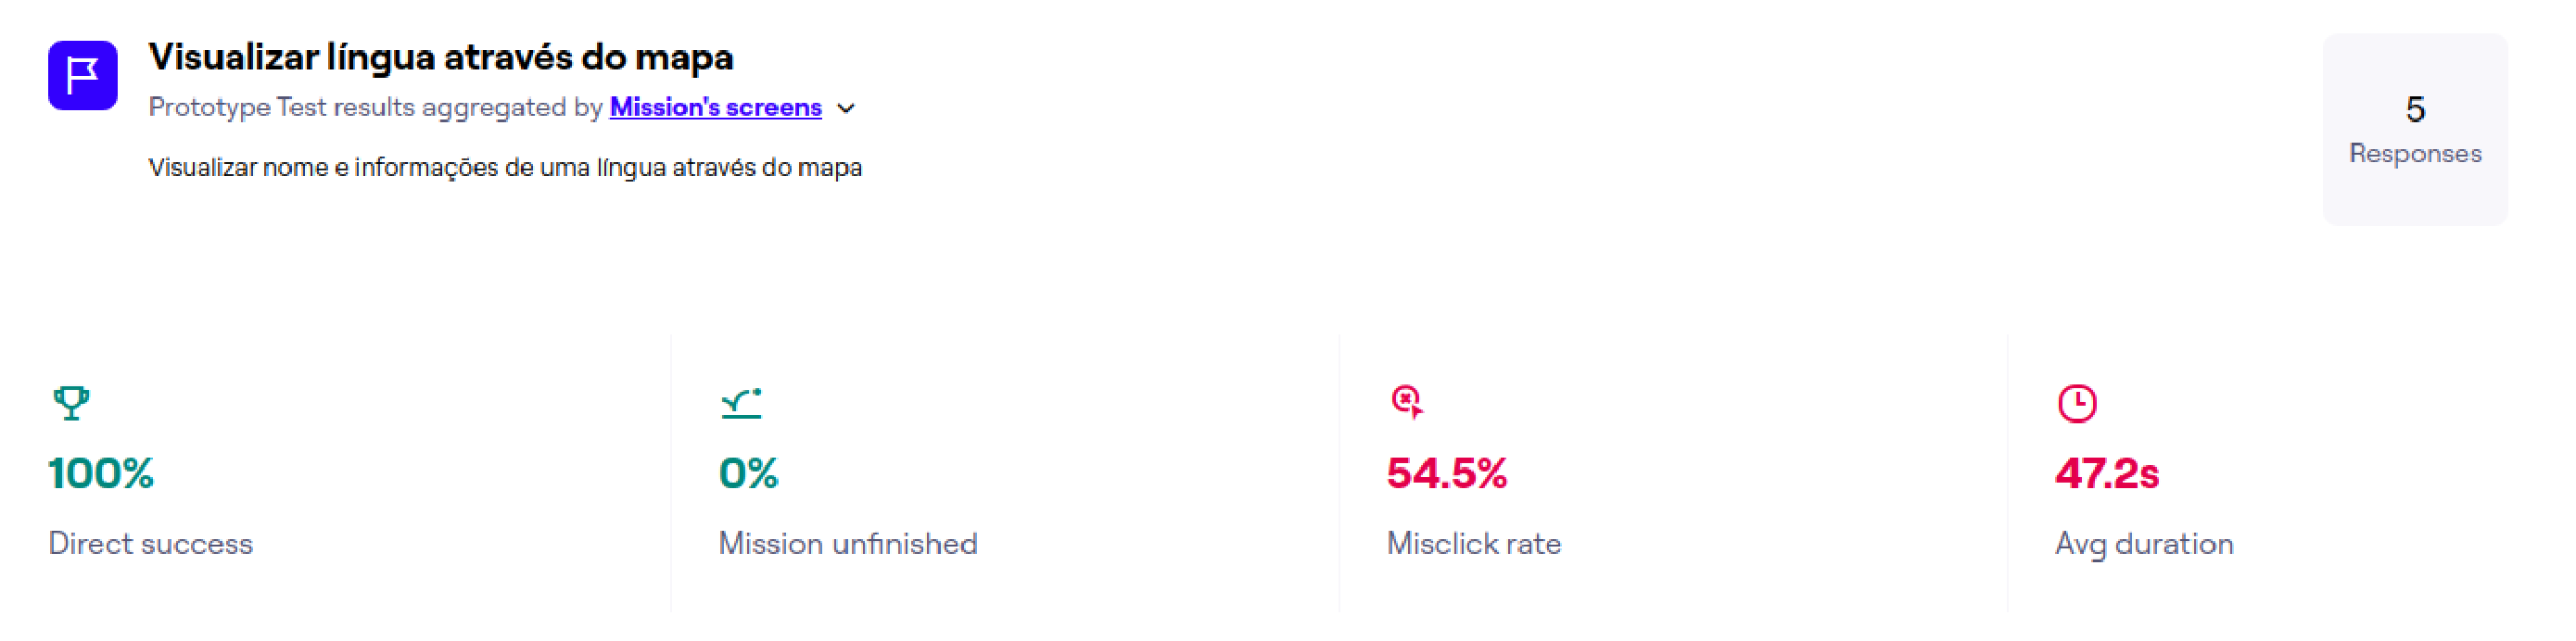
\includegraphics[width=1\textwidth]{figuras/maze.eps}
	\end{adjustbox}
	\begin{tablenotes}[flushleft]
		\centering
		\item \textit{Fonte:} Autora.
	\end{tablenotes}
	\label{fig31}
\end{figure}

A Figura \ref{fig32} fornece informações de sessão específicas por participante, incluindo o tempo gasto durante a execução das tarefas e o resultado obtido, indicando se foi um sucesso direto ou indireto.

O sucesso direto é caracterizado pela capacidade do participante de concluir a tarefa seguindo o caminho esperado, ou seja, o fluxo de telas definido para que o participante complete uma tarefa específica. Por outro lado, o sucesso indireto ocorre quando o usuário completa a tarefa 
sem seguir esse caminho previamente definido, seja passando por um fluxo diferente ou percorrendo um número maior de telas antes de concluir.

\begin{figure}[h!]
	\centering
	\caption{Resultados por participante na plataforma Maze}
	\begin{adjustbox}{center}
		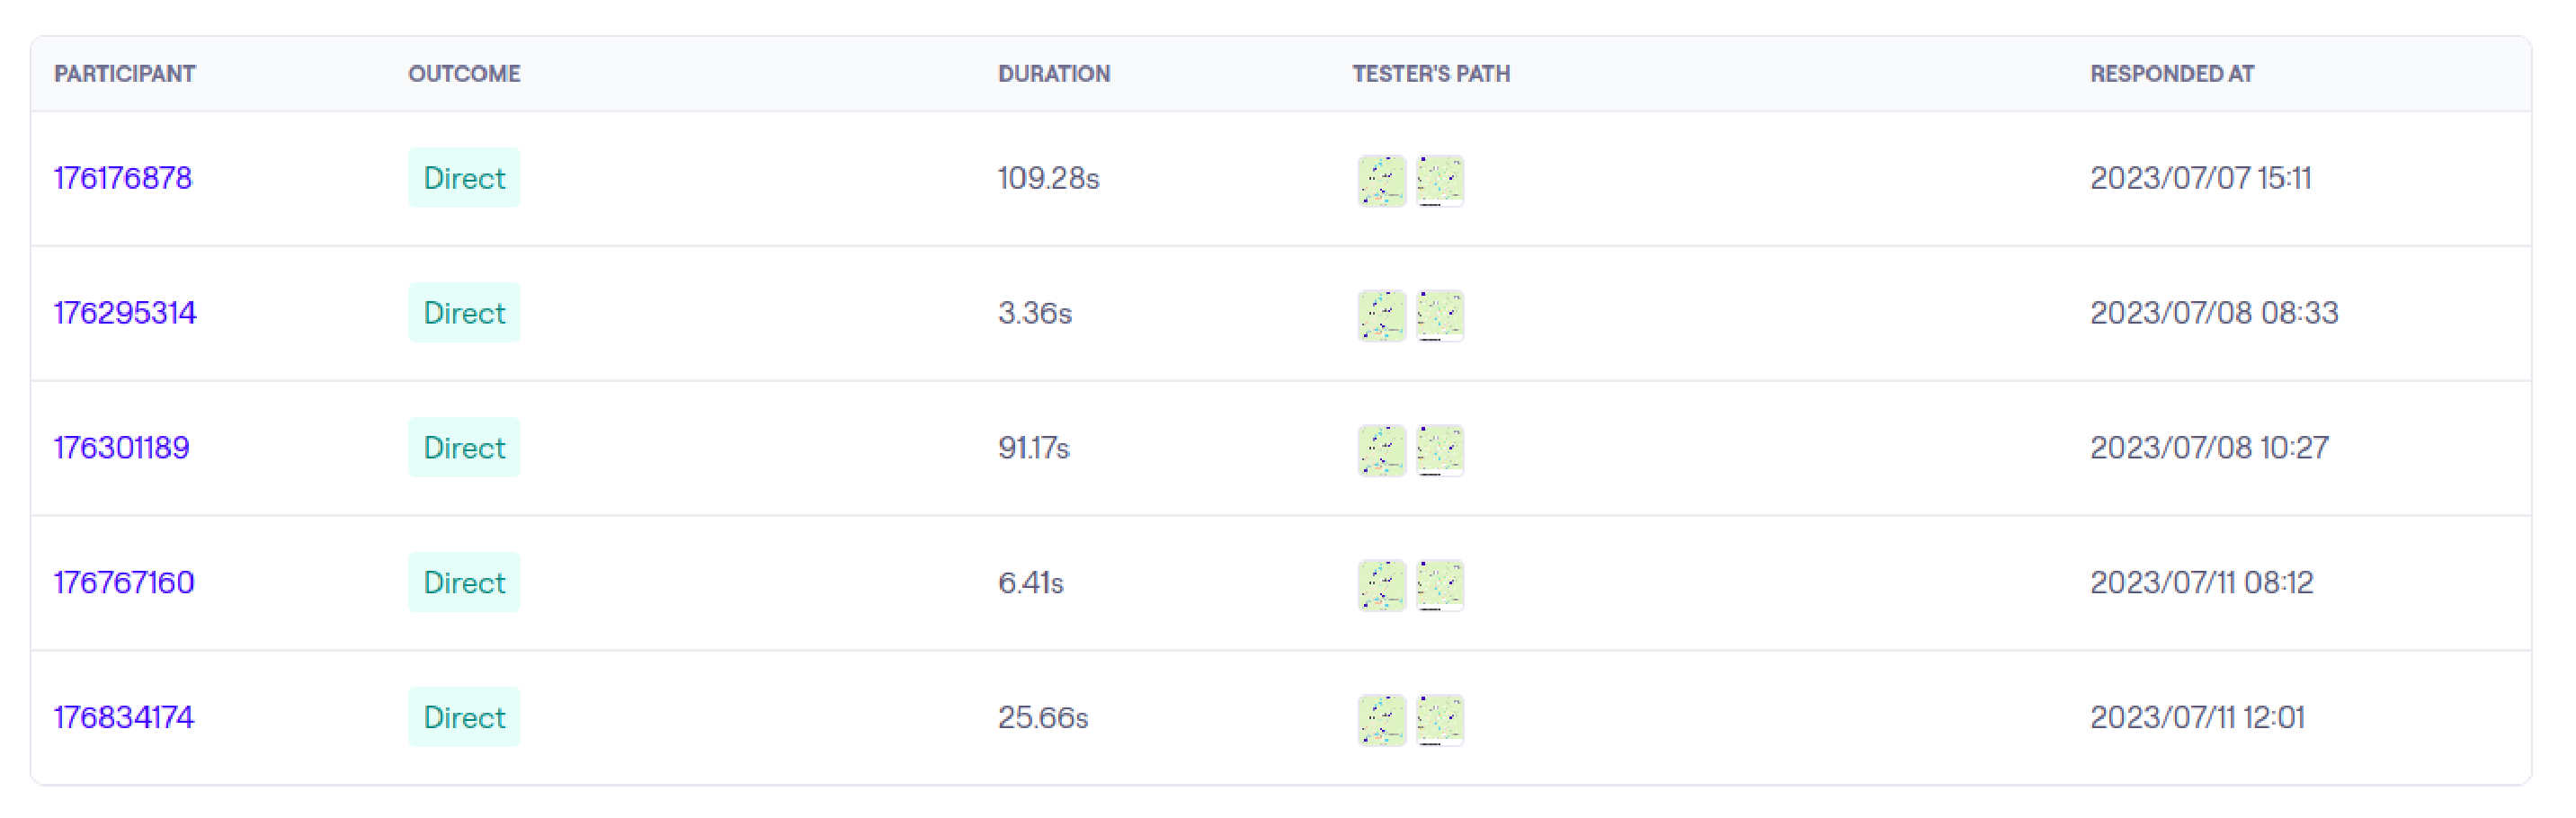
\includegraphics[width=1\textwidth]{figuras/maze2.eps}
	\end{adjustbox}
	\begin{tablenotes}[flushleft]
		\centering
		\item \textit{Fonte:} Autora.
	\end{tablenotes}
	\label{fig32}
\end{figure}

Além disso, ao final dos testes, foi aplicado um questionário baseado no Questionário \textit{Attrakdiff} para avaliar a experiência do usuário no aplicativo Multilind. Este questionário foi detalhadamente explicado na seção \hyperref[sec:Medicao2]{2.3.1}.

\section{Primeiro Ciclo de Testes}
\label{sec:Primeiro Ciclo}
O primeiro ciclo de testes foi conduzido com cinco usuários, com o objetivo de avaliar as funcionalidades na versão v1.4.0 do aplicativo. Durante esse ciclo, os participantes realizaram as tarefas enquanto forneciam \textit{feedback} instantâneo sobre suas experiências durante o uso 
do aplicativo. Os principais pontos levantados foram:

\begin{itemize}
	\item Falta de orientação no primeiro uso: foi observado pelos participantes a falta de instruções claras e orientações sobre como navegar e utilizar as funcionalidades no primeiro acesso ao aplicativo;
	\item Maior clareza na opção de visualizar línguas por família linguística: alguns participantes relataram dificuldades em localizar a opção para visualizar as línguas agrupadas por família linguística;
	\item Ausência de cores: usuários relataram sentir que a aplicação carecia de uma paleta de cores mais vibrantes para torná-la visualmente atraente, e
	\item Carência de informações a respeito de como contribuir: houve interesse manifestado por alguns participantes em contribuir com a base de dados do aplicativo. Entretanto, sentiram falta de informações a respeito 
	de como contribuir no aplicativo.
\end{itemize}

\subsection{Teste de Usabilidade}
\label{sec:Teste de Usabilidade}
A Tabela \ref{tab06} apresenta o tempo gasto por participante durante o teste de usabilidade separado por funcionalidade. Observa-se, com base nos dados expostos, que a F04 - Visualizar línguas por família linguística, 
demandou mais tempo, independentemente de quem estava testando. Por outro lado, as funcionalidades F01 - Visualizar línguas através do mapa, e F02 - Ver detalhes de uma língua ao clicar em um ponto no mapa, tiveram tempos 
de resposta mais baixos, o que indica que essas funcionalidades foram realizadas de forma mais eficiente pelos participantes.

\begin{table}[h!]
	\centering
	\caption{Tempo gasto por participante - Primeiro ciclo de testes}
	\label{tab06}
	\begin{adjustbox}{center}
	\begin{tabular}{l|l|l|l|l|l}
	\hline
	Fucionalidade & Participante 1 & Participante 2 & Participante 3 & Participante 4 & Participante 5 \\ 	\hline
	F01                   & 25.7s     & 109.3s     & 3.36s      & 232s       & 6.4s      \\
	F02                   & 21.2s        & 18.9s      & 6.45s      & 181.7s    & 17.2s     \\
	F03                   & 26.1s        & 25.7s      & 26.5s      & 36.9s     & 23.6s     \\
	F04                   & 69.6s        & 309.3s     & 283.2s     & 136.2s     & 193.9s     \\
	F05                   & 32.1s      & 31.4s      & 21.7s     & 72.6s     & 16.4s     \\
	F06                   & 30.7s     & 8.4s      & 24s     & 45.7s     & 75.5s     \\
	F07                   & 43.2s     & 23.8s      & 43.5s     & 181.2s    & 35s      \\ 	\hline
	\end{tabular}
	\end{adjustbox}
	\begin{tablenotes}[flushleft]
		\centering
		\item \textit{Fonte:} Maze. Disponível em: \url{https://app.maze.co/report/Multilind/3nsxpiljsgn073/intro}.
	  \end{tablenotes}
\end{table}

\subsection{Teste de Experiência de Usuário}
\label{sec:Teste de Experiência de Usuário}
Após a conclusão dos testes de usabilidade, os participantes preencheram o Questionário \textit{Attrakdiff}, a fim de 
avaliar a experiência, qualidade e usabilidade da aplicação. Dada a maior abrangência de informações conferidas pelo Questionário \textit{Attrakdiff}, optou-se por representar esses dados em uma tabela disponível no Google Sheets, que pode ser acessada via o link: 
\url{https://docs.google.com/spreadsheets/d/1zVGAgqTqRUIRba0kFmWySBV_MLnNHqAVeRMLFGzIHLE/edit?usp=sharing}. 

Com base nos resultados desse questionário, foi elaborado um gráfico (Figura \ref{fig20}), em que é possível ter uma visão geral da pontuação alcançada em cada par de palavras avaliadas. Analisando os dados obtidos, percebe-se que os pares de palavra-chave mais bem conceituados foram: "Incontrolável - Gerenciável''; "Sem imaginação - Criativo'', e "De baixa qualidade - De alta qualidade''. 
Tais pares de palavras pertencem às dimensões Qualidade Pragmática Percebida; Qualidade da Experiência Hedônica Estímulo, e Qualidade Hedônica-Identidade, respectivamente. A explicação acerca das dimensões 
pode ser conferida na seção \hyperref[sec:Medicao2]{2.3.1}. 

\begin{figure}[h!]
	\centering
	\caption{Média Geral \textit{Attrakdiff} - Primeiro Ciclo de Testes}
	\begin{adjustbox}{center}
		\includegraphics[width=1\textwidth]{figuras/media-geral.eps}
	\end{adjustbox}
	\begin{tablenotes}[flushleft]
		\centering
		\item \textit{Fonte:} Autora.
	\end{tablenotes}
	\label{fig20}
\end{figure}

Já os pares de palavra-chave que revelaram menor satisfação foram: "Cauteloso - Ousado'' e "Confuso - Bem Estruturado''. Isso indica que os participantes perceberam o sistema como mais cauteloso do que ousado, e 
sentiram-se confusos na interação com o sistema. Em suma, e considerando esses \textit{feedbacks}, foi identificado que é necessário focar nas seguintes melhorias: fornecer mais orientações, aprimorar a 
organização e garantir clareza nas informações apresentadas. As Figuras \ref{fig20} e \ref{fig21} ilustram, respectivamente, a média de respostas geral e a média de respostas separadas pelas quatro dimensões principais. 

Ressalta-se que, na média (Figura \ref{fig20}), há aspectos que chamam atenção por seus extremos. "Cauteloso - Ousado'' foi avaliado pelos participantes, obtendo 4,4 como média. Já "Desencorajador - Motivador'' foi avaliado pelos 
participantes com média 6,4. Ao que indica, o aplicativo Multilind pode ser melhorado em "Cauteloso - Ousado''. Já "Desencorajador - Motivador'', em um primeiro momento, não é uma prioridade nas melhorias. Para maior conforto 
quanto à análise dos dados, ressalta-se que valores mais altos, em um intervalo de 0 a 7, representam maior concordância por parte dos participantes no tópico questionado na pergunta, e o inverso é verdadeiro. Na Figura \ref{fig21}, 
reporta-se sobre a maior satisfação dos usuários na dimensão Atratividade, com média na dimensão em 6,15. Em oposição, têm-se as dimensões: Qualidade de Estimulação (Henônica), com média na dimensão em 5,2 (a menor dentre 
as quatro dimensões), e Qualidade Pragmática Percebida, com média na dimensão em 5,48 (segunda menor dentre as quatro dimensões).

\begin{figure}[h!]
	\centering
	\caption{Média \textit{Attrakdiff} por dimensões - Primeiro Ciclo de Testes}
	\begin{adjustbox}{center}
		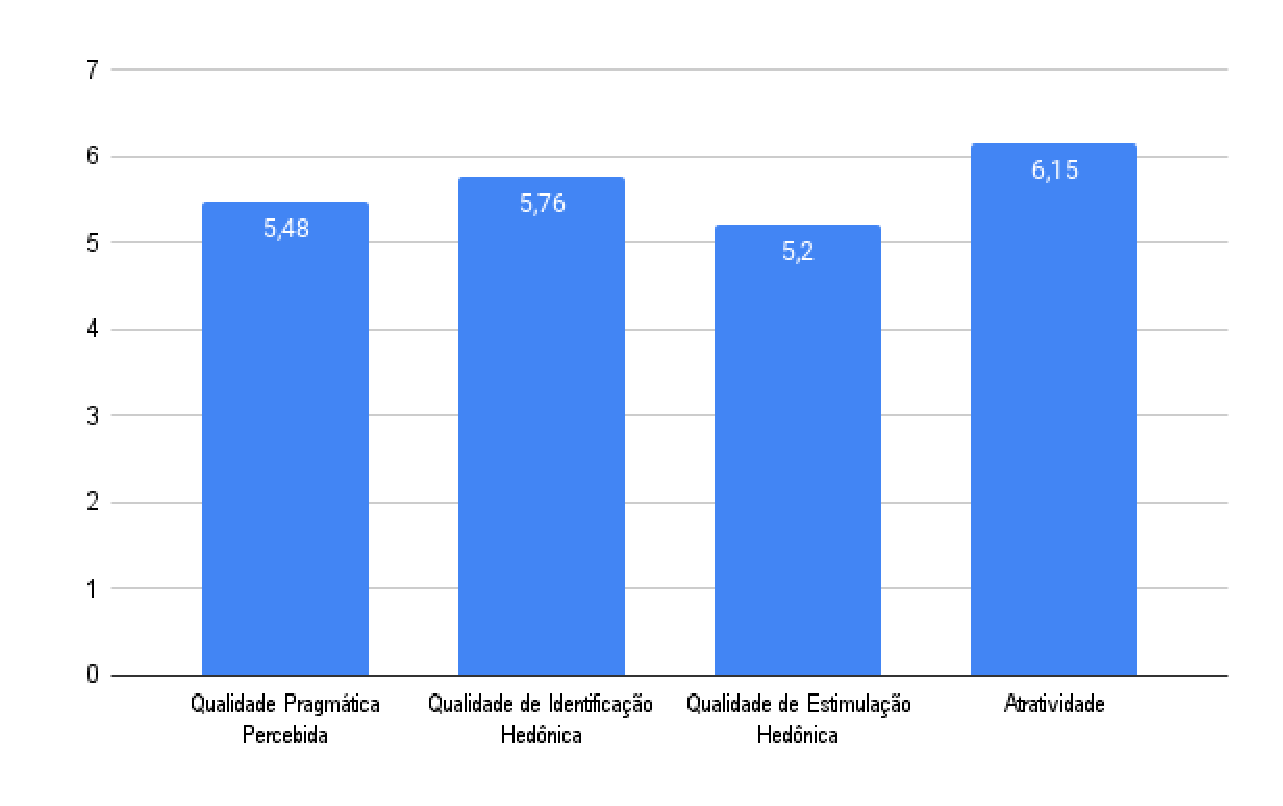
\includegraphics[width=1\textwidth]{figuras/media-separada.eps}
	\end{adjustbox}
	\begin{tablenotes}[flushleft]
		\centering
		\item \textit{Fonte:} Autora.
	\end{tablenotes}
	\label{fig21}
\end{figure}